\scanpage{28}
\mspage{14}
groupes fondamentaux sont \inserted{en apparence} triviaux :
\[
\pi_1(\mathcal T_{0\nu})=0\qquad 0\leq\nu\leq3
\]
Le Topos $\mathcal T_{0,\nu}$ \deleted{est le \inserted{gros} topos fibré} \inserted{$(\nu\geq4)$ correspond au} \deleted{étale de} \inserted{schéma} des syst. de $\nu-3$ points distincts $(x_1,\ldots,x_{\nu-3})$ dans
\[
\mathbf P^1-\{0,1,\infty\}=\mathbf E^1\setminus\{0,1\}.
\]
Son groupe fondamental est 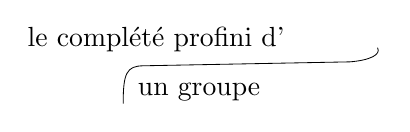
\begin{tikzpicture}[baseline=(base.base)]
\node[anchor=base west,inner sep=0] (base) at (0,0) {un groupe};
\node[anchor=base west,inner sep=0] at (-1.4,.62) {\inserted{le complété profini d'}};
\draw[line width=.3pt] (-.18,-.10) .. controls (-.18,.28) and (-.14,.38) .. (.08,.38) -- (2.7,.43) .. controls (2.95,.45) and (3.1,.52) .. (3.05,.61);
\end{tikzpicture} de tresses $\Pi_{0,\nu}$, lequel (en tant que ``groupe extérieur'') dépend contra-fonctoriellement de $[1,\nu]$ pour les monomorphismes.

Sur $(\mathcal T_{0,\nu})_{\mathbf Q}$ \inserted{du $(\mathcal T_{\unsure{0\nu|0,\nu}})_{\overline{\mathbf Q}}$} on fait opérer $\mathfrak S_\nu$, donc $\mathfrak S_\nu\times\Gamma$ opère sur $\mathcal T_{0,\nu}$,
\figure{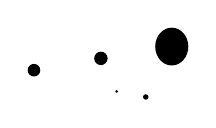
\begin{tikzpicture}[x=1cm,y=1cm]
\fill (0,0) circle (.08);
\fill (.85,.15) circle (.085);
\fill (1.75,.3) ellipse (.21 and .24);
\fill (1.05,-.27) circle (.018);
\fill (1.42,-.34) circle (.035);
\end{tikzpicture}}
\mspage{27}
